
To communicate with a computer, one is required to 'speak' the same language as the computer. A computer's language is pre-defined by the producer of the computer, and generally referred to as \emph{machine code} or \emph{machine instructions}.\\
Today software developers make use of various programming languages. Each language deals with an area of functionality. These languages have to be translated for the computer and this is done with tools called compilers.\\
When developing, the choice of programming language can be vital to the project's success and functionality.\\\\
In this report, a description of the development-process of a new language is laid out.

\section{\langname{}}
In this project we want to address the interest for a role-playing based language. The purpose of the language is to define characters, skills, attributes, effects etc,  found in various role-playing games.\\
To do this we construct a language which should catch the intuitive and simple characteristics of character sheets, which are information containers for various role-playing games.

\section{Role-playing}
Role-playing games have been around for some time now and exist in many forms.
These include \emph{Computer role-playing}- and \emph{Pen \& Paper role-playing-games}, both a focus in this project.\\
In role-playing games, players take on the roles of fictitious characters, either created by the players themselves or by the developers of the game.\\
Characters are defined by their abilities and attributes, meaning that everything that matters gets assigned a number to represent how 'good' an ability or an attribute is. In \emph{Pen \& Paper games} a character is not much more than an idea built around various numbers, these numbers representing everything that matters in the given world.\\ For example the strength and charisma of a character can tell you how hard a character can hit and how well they can handle social situations. Most games however break as much as possible down to numbers; appearance, intellect, luck and more.
This should in a way contribute to the level of realism in events and outcomes while playing.\\
The first modern \emph{Pen \& Paper role-playing game} to be released commercially is the game \emph{Dungeons \& Dragons}, which was first published in 1974.\cite{wikidnd}
\emph{Dungeons \& Dragons} can therefore be thought of as the pioneer of role-playing games.
\subsection*{Pen \& Paper}
When playing \emph{Pen \& Paper games} the players generally use dice (see figure \vref{dice}) to determine an outcome of an activity, for example could this activity be an attack, where the outcome determines if the attack is successful and thereafter how much damage is inflicted. To help keep track of a character's attributes and other information, a character sheet is used.
A game scenario can be described as following: A game master prepares an adventure for the players, participants are seated around a table, in each participant's possession is a writing tool, character sheet (printed on a piece of paper) and a number of dices. Each player creates a character to use in the given adventure, when everyone is ready the adventure starts and the game master describes the setting and series of events. When an action is required from a specific player, he can determine the outcome of the action by rolling a specific set of dice. In an event where 2 or more players are included, participants roll for initiative, meaning that they roll to see in what order they can take action.
\begin{figure}[!h]
\centering
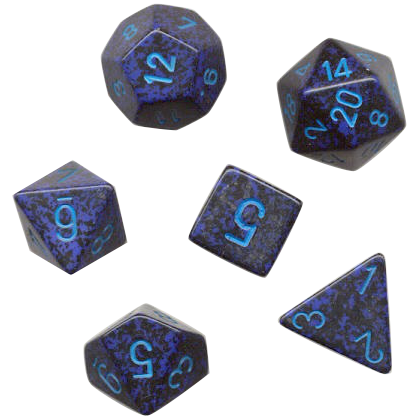
\includegraphics[scale=0.4]{img/rpgdice.png}
\caption{Dice for role-playing purposes}
%\cite{rpgdice}
\label{dice}
\end{figure}
\subsection*{Digitised}
In \emph{Computer role-playing games} the outcome of an activity is determined by measures implemented by the developers, this can be an imitation of a dice roll (variation) or a static calculation (pre-calculated).
To keep track of character information, a digitised character sheet is often accessible, where the player can customise his character to some degree.\\
Due to the increasing popularity of role-playing games, the benefit of a role-playing based programming language becomes greater.
\pagebreak

%source: (wikidnd) http://en.wikipedia.org/wiki/History_of_role-playing_games